\section{Quotient Groups and Homomorphisms}

\subsection{Definitions and Examples} \label{sec3.1}

\defi Let $\phi : G \to H$ be a homomorphism. The \textbf{kernel} of $\phi$ is the set
\[\ker\phi = \{g \in G \mid \phi(g) = 1\}\]
where $1_H$ is the identity of $H$. The \textbf{image} of $\phi$ is the set
\[\im\phi = \{\phi(g) \mid g \in G\}\]

\prop[Homomorphism Properties] \label{prop3.1}
Let $\phi : G \to H$ be a group homomorphism. Then
\begin{enumerate}
    \item $\phi(1_G) = 1_H$, where $1_G$ and $1_H$ are the identities of $G$ and $H$, respectively.
    \item $\phi(g\inv) = \phi(g)\inv$ for every $g \in G$.
    \item $\phi(g^n) = \phi(g)^n$ for every $n \in \z$.
    \item $\ker\phi \leq G$.
    \item $\im\phi \leq H$.
\end{enumerate}

\begin{proofnum}
    \item $\phi(1_G) = \phi(1_G1_G) = \phi(1_G)\phi(1_G)$. By cancellation, $1_H = \phi(1_G)$.
    \item $1_H = \phi(1_G) = \phi(gg\inv) = \phi(g)\phi(g\inv)$ for all $g \in G$. Then $\phi(g)\inv = \phi(g\inv)$.
    \item For $n = 0$, the result is (i). Using induction for $n \in \zp$, use (ii) for $n < 0$.
    \item Note $1_G \in \ker\phi$. Suppose $x, y \in \ker\phi$. Then $\phi(xy\inv) = \phi(x)\phi(y\inv) = 1_H1_H\inv = 1_H$ so that $xy\inv \in \ker\phi$.
    \item Note $1_H \in \im\phi$. Suppose $x, y \in \im\phi$. Then there exists $g, h \in G$ such that $\phi(g) = x$ and $\phi(h) = y$. Then $xy\inv = \phi(g)\phi(h\inv) = \phi(gh\inv)$. Since $gh\inv \in G$, then $xy\inv \in \im\phi$.
\end{proofnum}

\defi Let $\phi : G \to H$ be a homomorphism with kernel $K$. The \textbf{quotient group} $G/K$ is the group whose elements are the fibers of $\phi$ with operation as such: if $X = \phi\inv(a)$ and $Y = \phi\inv(b)$ for $a, b \in H$, then $XY = \phi\inv(ab)$.

\prop[Translates of a Kernel] \label{prop3.2}
Let $\phi : G \to H$ be a homomrphism with kernel $K$. Let $X = \phi\inv(a)$ for $X \in G/K$. Then
\begin{enumerate}
    \item For any $x \in X$, $X = \{xk \mid k \in K\}$.
    \item For any $x \in X$, $X = \{kx \mid k \in K\}$.
\end{enumerate}

\begin{proofnum}
    \item Let $x \in X$, hence $\phi(x) = a$. Let $xK = \set{xk \mid k \in K}$. For any $k \in K$, then $xk \in X$, or $xK \subseteq X$. If $y \in X$, put $k = x\inv y$. Then $k \in K$ so that $y = xk \in xK$, hence $X \subseteq xK$.
    \item Define $Kx = \set{kx \mid k \in K}$. The proof follows similarly as (i), except we set $k = yx\inv$ so that $kx = y \in X$, hence $X \subseteq Kx$.
\end{proofnum}

\defi Let $N \leq G$ and $g \in G$. The \textbf{left coset} and \textbf{right coset} of $N$ in $G$ are the sets
\[gN = \{gn \mid n \in N\}, \quad Ng = \{ng \mid n \in N\}.\]
Elements of a coset are called \textbf{representatives}.

\theo[Coset Multiplication] \label{theo3.3}
Let $G$ be a group with $K$ a kernel of some homomorphism from $G$ to another group. The set of left cosets of $K$ in $G$ with operation
\[aK \circ bK = (ab)K\]
forms the group $G/K$. This operation is well defined in that if $a' \in aK$ and $b' \in bK$, then $a'b' \in abK$, and $a'b'K = abK$. This is also analogously defined for right cosets.
\begin{proof}
    Let $X, Y \in G/K$ with $Z = XY \in G/K$. Then $X, Y, Z$ are left cosets of $K$. Since $K$ is the kernel of a homomorphism, then $X = \phi\inv(a)$ and $Y = \phi\inv(b)$ for $a, b \in H$. Moreover, $Z = \phi\inv(ab)$. Let $x \in X$ and $y \in Y$ so that $\phi(x) = a$ and $\phi(y) = b$. Then $X = xK$ and $Y = yK$. Then $xy \in Z$ if and only if $xy \in \phi\inv(ab)$, or $\phi(x)\phi(y) = ab$, hence $Z = xyK$. Exercise 3.1.2 shows the other direction. Lastly, \autoref{prop3.2} shows that $xK = Kx$ and $yK = Ky$ for every $x, y \in G$.
\end{proof}

\newpage

\note Using similar notation from $\intmod$, we denote $G/K = \bar G$ with $\bar g = gK$ and $\bar g \bar h = \bar{gh}$.

\prop[Set of Cosets is Partition, Equivalency Criterion of Cosets] \label{prop3.4}
Let $N \leq G$. The set of left cosets of $N$ in $G$ form a partition of $G$. Moreover, for all $g, h \in G$, then $gN = hN$ if and only if $h\inv g \in N$. In particular, $gN = hN$ if and only if $g$ and $h$ represent the same coset.

\begin{proof}
    It is clear that $g \in gN$ for every $g \in G$. If $gN \cap hN$ is nonempty, let $k \in gN \cap hN$. Then $k = gn_1 = hn_2$ for $n_1, n_2 \in N$. Note that $g = kn_1\inv = hn_2n_1\inv$ where $n_2n_1\inv \in N$ since $N \leq G$. Then for any $gn \in gN$ for some $n \in N$, we have $gn = hn_2n_1\inv n \in hN$ so that $gN \subseteq hN$. A similar argument shows that $hN \subseteq gN$, hence they are equal, so that the cosets are either distinct or equal.

    The preceding argument shows $gN = hN$ if and only if $g \in hN$, or $g = hn$, or $h\inv g \in N$. Moreover, $h \in gN$ implies that $h$ is a representative of $gN$, so that $hN = gN$ if and only if $g$ and $h$ represent the same coset.
\end{proof}

\prop[Coset Multiplication, Extended] \label{prop3.5}
Let $G$ be a group with $N \leq G$.
\begin{enumerate}
    \item The operation $\cdot$ on the set of left cosets of $N$ in $G$ described by
    \[aN \cdot bN = (ab)N\]
    is well defined if and only if $gng\inv \in N$ for every $g \in G$ and $n \in N$.
    \item Well definedness of the above operation implies that the set of left cosets of $N$ in $G$ forms a group with identity $1N = N$ and inverse of $gN$ given by $(gN)\inv = g\inv N$.
\end{enumerate}

\begin{proofnum}
    \item Suppose the operation is well defined, and let $g \in G$ and $n \in N$. Then $g\inv N = ng\inv N$. Since $1 \in N$, then $ng\inv 1 \in ng\inv N$ so that $ng\inv = g\inv n'$ for some $n' \in N$. Then $gng\inv \in N$.
    
    If $gng\inv \in N$ instead for every $g \in G$ and $n \in N$, let $a, a_0 \in aN$ and $b, b_0 \in bN$ so that $a_0 = an$ and $b_0 = bm$ for some $n, m \in N$. Then
    \[a_0b_0 = (an)(bm) = a(nb)m = a(bn')m\]
    where we note that $nb = b(n')$ for some $n' \in N$ by assumption. Then $a_0b_0 \in abN$ so that $a_0b_0N \cap abN$ is nonempty. By \autoref{prop3.4}, then $a_0b_0N = abN$, hence the operation is well defined.
    \item Trivial verification using the prior proposition and the fact that $G$ is a group.
\end{proofnum}

\defi Let $N \leq G$ for group $G$.
\begin{itemize}
    \item For $n \in N$, the \textbf{conjugate} of $n$ by $g$ is the element $gng\inv$.
    \item The \textbf{conjugate} of $N$ by $g$ is the set $gNg\inv = \{gng\inv \mid n \in N\}$.
    \item We say some $g \in G$ \textbf{normalizes} $N$ if $gNg\inv = N$.
    \item We say $N$ is a \textbf{normal subgroup} of $G$, denoted by $N \nsub G$, if $gNg\inv = N$ for every $g \in G$. Equivalently, $N$ is normal if and only if every element of $G$ normalizes $N$.
\end{itemize}

\theo[Characterizations of Normal Subgroups] \label{theo3.6}
Let $G$ be a group with $N \leq G$. Then the following are equivalent:
\begin{enumerate}
    \item $N \nsub G$,
    \item $N_G(N) = G$,
    \item $gN = Ng$ for every $g \in G$,
    \item the operation on left cosets of $N$ in $G$ described in \autoref{prop3.5} makes the set of left cosets into a group,
    \item $gNg\inv \subseteq N$ for every $g \in G$.
\end{enumerate}

\begin{proof}
    \leavevmode
    \begin{itemize}
        \item (i) if and only if (ii) by definition of normality and normalizer.
        \item (ii) if and only if (iii), since $gNg\inv = N$ implies $gN = Ng$ for every $g \in G$.
        \item (iii) implies (iv) by \autoref{prop3.5}.
        \item (iv) implies (v), as well definedness of the operation implies $gng\inv \in N$ for every $g \in G$ and $n \in N$ by \autoref{prop3.5}.
        \item (v) implies (i), because $g\inv Ng \subseteq N$ in particular, hence $N \subseteq gNg\inv \subseteq N$ so that $gNg\inv = N$ for every $g \in G$.
    \end{itemize}
\end{proof}

\prop[Normal Subgroup Are Kernels] \label{prop3.7}
$N \nsub G$ if and only if $N = \ker\phi$ for some homomorphism $\phi$ on $G$.
\begin{proof}
    If $N \nsub G$, let $\pi : G \to G/N$ be the map
    \[\pi(g) = gN, \quad g \in G\]
    It is clear that $\pi$ is a homomorphism. Moreover, $\pi(g) = 1N$ when $gN = N$, or $g \in N$, hence $\ker\pi = N$.

    If $N$ is instead a kernel of some homomorphism, then $gN = Ng$ for $g \in G$ by \autoref{prop3.2}. Then $N \nsub G$ by \autoref{theo3.6}.
\end{proof}

\defi For $N \nsub G$, then the homomorphism $\pi : G \to G/N$ given by $\pi(g) = gN$ is called the \textbf{natural projection homomorphism} from $G$ to $G/N$. Moreover, for $\bar H \leq G/N$, the set $\pi\inv(\bar H)$ is the \textbf{complete preimage} of $\bar H$ in $G$.

\note We claim quotient groups of cyclic groups are cyclic. Let $G = Z_n$ for some $n \in \zp$ with $g \in G$ such that $\gen g = G$. For some $N \leq G$, we know $N = \gen{g^d}$ for smallest positive integer $d$ such that $g^d \in N$. Note that $g^\alpha N = (gN)^\alpha$ for every $\alpha \in \z$ by Exercise 3.1.4, hence $G/N = \gen{gN}$. By Exercise 3.1.5, we know $|gN| = d$, and $d = |G|/|N|$ by \autoref{prop2.5}, so that $G/N \cong Z_d$.
\newpage

\subsection{More on Cosets and Lagrange's Theorem} \label{sec3.2}

\theo[Lagrange's Theorem] \label{theo3.8}
Let $G$ be a finite group with $H \leq G$. Then $|H|$ divides $|G|$. Also, the number of left cosets of $H$ in $G$ is $|G|/|H|$.
\begin{proof}
    Let $|H| = n$ and let $k$ be the number of left cosets of $H$ in $G$. \autoref{prop3.4} shows that these cosets partition $H$, and the map $H \to gH$ given by $h \mapsto gH$ is a bijection for every $g \in G$, hence each coset has $n$ elements. Since the cosets partition $G$, then $|G| = kn$, so that $n$ divides $|G|$ and the number of left cosets is $k = |G|/n$.
\end{proof}

\defi Let $G$ be a (possibly infinite) group with $H \leq G$. The \textbf{index} of $H$ in $G$ is the number of left cosets of $H$ in $G$, denoted by $|G : H|$.

\cor[Element Order Divides Group Order] \label{cor3.9}
Let $G$ be a finite group and let $g \in G$. Then the order of $g$ divides the order of $G$. In particular, $g^{\abs G} = 1$.
\begin{proof}
    \autoref{prop2.2} shows that $\abs g = \abs{\gen x}$. Then the first part follows by using Lagrange's Theorem on $H = \gen g$. Since $\abs G$ is a multiple of $\abs g$, the second part follows.
\end{proof}

\cor[Prime Order Implies Cyclic] \label{cor3.10}
Let $G$ be a group of prime order. Then $G \cong Z_p$ for some prime $p$.
\begin{proof}
    For non-identity $g \in G$, then $\gen g \leq G$ is nontrivial, hence $\gen g = G$ by the primality of $|G|$. Then $G$ is cyclic, and $G \cong Z_{|G|}$ by \autoref{theo2.4}.
\end{proof}

\note We claim $H \nsub G$ when $|G : H| = 2$. For $g \in G - H$, then $G/H = \set{1H, gH} = \set{H1, Hg}$. Since $H = 1H = H1$, then $gH = G - H = Hg$, hence $H \nsub G$ by \autoref{theo3.6}.

\theo[Cauchy's Theorem] \label{theo3.11}
Let $G$ be finite with prime $p$ dividing $|G|$. Then there exists $g \in G$ where $|g| = p$.

\theo[Sylow] \label{theo3.12}
Let $G$ be finite with $|G| = p^nm$ such that $p$ is prime and $p \nmid m$. Then there exists $H \leq G$ such that $|H| = p^n$.

\defi Let $H, K \leq G$. The \textbf{subgroup product} of $H$ and $K$ is the set
\[HK = \{hk \mid h \in H, k \in K\}\]

\prop[Cardinality of Subgroup Product] \label{prop3.13}
Let $H$ and $K$ be subgroups of a finite group $G$. Then
\[|HK| = \frac{|H||K|}{|H \cap K|}\]
\begin{proof}
    Observe $HK$ is a union of left cosets of $K$. To find the number of distinct left cosets of the form $hK$ for $h \in H$, observe that $h_1K = h_2K$ for some $h_1, h_2 \in H$ if and only if $h_2\inv h_1 \in K$, or $h_2\inv h_1 \in H \cap K$. Then the number of distinct left cosets of $K$ in $HK$ is $|H : H \cap K| = |H|/|H \cap K|$. The result follows by noting that each coset has $|K|$ elements.
\end{proof}

\prop[Characterization of Subgroup Product as a Subgroup] \label{prop3.14}
If $H, K \leq G$, then $HK \leq G$ if and only if $HK = KH$.
\begin{proof}
    If $HK \leq G$, we have $KH \subseteq HK$ from $H, K \leq HK$. For $hk \in HK$, then $hk = (h_0k_0)\inv = k_0\inv h_0\inv \in KH$ for some $h_0 \in H$ and $k_0 \in K$, hence $HK \subseteq KH$.

    If $HK = KH$, let $a, b \in HK$ with $a = h_1k_1, b = h_2k_2$ for $h_i \in H$ and $k_i \in K$. Then $ab\inv = h_1k_1k_2\inv h_2\inv \in HK$. Since $KH = HK$, $(k_1k_2\inv) h_2\inv = h_3k_3$ for some $h_3 \in H$ and $k_3 \in K$, hence $ab\inv = h_1h_3k_3 \in HK$, or $HK \leq G$.
\end{proof}

\cor[Normalizing Criterion for Subgroup Products] \label{cor3.15}
Let $H, K \leq G$ with $H \leq N_G(K)$. Then $HK \leq G$. In particular, $K \nsub G$ implies $HK \leq G$ for every $H \leq G$.

\begin{proof}
    Observe $khk\inv in K$ for all $h \in H$ and $k \in K$ by assumption. Then $hk = (hkh\inv)h \in KH$, and $kh = h(h\inv kh) \in HK$ for all $h \in H$ and $k \in K$, hence $HK = KH$. By \autoref{prop3.14}, then $HK \leq G$.
\end{proof}

\defi Let $A \subseteq N_G(K)$ or $C_G(K)$. Then $A$ \textbf{normalizes}, or \textbf{centralizes} $K$, respectively.

\newpage

\subsection{The Isomorphism Theorems} \label{sec3.3}

\theo[The First Isomorphism Theorem] \label{theo3.16}
If $\phi : G \to H$ is a group homomorphism, then $\ker\phi \nsub G$ and $G/\ker\phi \cong \phi(G)$.
\begin{proof}
    Note that $\ker\phi \nsub G$ by \autoref{prop3.7}. Consider the map
    \[\psi : G/\ker\phi \to \phi(G), \quad g\ker\phi \mapsto \phi(g),\]
    and also observe that $\phi = \psi \circ \pi$ where $\pi$ is the natural projection homomorphism. To show that $\psi$ is well defined, observe that $g\ker\phi = h\ker\phi$ implies $h\inv g \in \ker\phi$, or $\phi(h) = \phi(g)$. The backwards shows injectivity, and surjectivity is clear by definition of $\phi(G)$. A composition of homomorphisms is a homomorphism, hence $\psi$ is an isomorphism from $G/\ker\phi$ to $\phi(G)$.
\end{proof}

\cor[Consequences of the First Isomorphism Theorem] \label{cor3.17}
Let $\phi : G \to H$ be a group homomorphism. Then
\begin{enumerate}
    \item $\phi$ is injective if and only if $\ker\phi = 1$, and
    \item $|G : \ker\phi| = |\phi(G)|$.
\end{enumerate}

\begin{proofnum}
    \item If $\phi$ is injective, then $\phi(g) = 1$ implies $g = 1$. Conversely, a trivial kernel implies for any $g, h \in G$ such that $\phi(g) = \phi(h)$ that $\phi(h\inv g) = 1$, hence $h\inv g = 1$ or $g = h$.
    \item By the First Isomorphism Theorem, then $G/\ker\phi \cong \phi(G)$, so that $|G : \ker\phi| = |G/\ker\phi| = |\phi(G)|$.
\end{proofnum}

\theo[The Second (Diamond) Isomorphism Theorem] \label{theo3.18}
Let $G$ be a group with $A, B \leq G$ and $A \leq N_G(B)$. Then $AB \leq G$, $B \nsub AB$, $A \cap B \nsub A$, and $AB/B \cong A/A \cap B$. A diagram of the subgroup lattice is as follows:
\begin{center}
    \begin{tikzpicture}[scale=1.1]
        \node (G) at (0, 0) {$G$};
        \node (AB) at (0, -1) {$AB$};
        \node (A) at (-1, -2) {$A$};
        \node (B) at (1, -2) {$B$};
        \node (AintB) at (0, -3) {$A \cap B$};
        \node (1) at (0, -4) {$1$};

        \draw (1) -- (AintB) -- (A) -- (AB) -- (G);
        \draw (AintB) -- (B) -- (AB);
    \end{tikzpicture}
\end{center}

\begin{proof}
    \autoref{cor3.15} shows that $AB \leq G$. Also, $AB \leq N_G(B)$, or $B \nsub AB$. Consider $\pi |_A : AB \to AB/B$. Then $\ker\pi|_A$ consists of elements $a \in A$ such that $aB = B$, or $a \in B$, hence $a \in A \cap B$. By the First Isomorphism Theorem, then $A \cap B \nsub A$ and $A/A \cap B \cong AB/B$.
\end{proof}

\theo[The Third Isomorphism Theorem] \label{theo3.19}
Let $G$ be a group with $N_1 \nsub G$ and $N_2 \nsub G$ such that $N_1 \leq N_2$. Then $N_2/N_1 \nsub G/N_1$ and
\[(G/N_1)/(N_2/N_1) \cong G/N_2.\]
\begin{proof}
    It is clear that $N_2/N_1 \nsub G/N_1$ by $N_2 \nsub G$. The map
    \[\phi : G/N_1 \to G/N_2, \quad gN_1 \mapsto gN_2\]
    is well defined, since $N_1 \leq N_2$. It is easy to see that $\phi$ is a surjective homomorphism. Moreover, $\phi(gN_1) = N_2$ if and only if $gN_2 = N_2$, or $g \in N_2$, hence $\ker\phi = N_2/N_1$. The First Isomorphism Theorem finishes the proof.
\end{proof}

\theo[The Fourth (Lattice) Isomorphism Theorem] \label{theo3.20}
Let $G$ be a group with $N \nsub G$. Then every subgroup of $\bar G$ is of the form $\bar A$ for some $A \leq G$ with $N \leq A$, and $A \mapsto \bar A$ is a bijection from the set of subgroups of $G$ containing $N$ to the set of subgroups of $\bar G$. This bijection has the following properties:
\begin{enumerate}
    \item $A \leq B$ if and only if $\bar A \leq \bar B$,
    \item $A \leq B$ implies $[B : A] = [\bar B : \bar A]$,
    \item $\bar{\gen{A, B}} = \gen{\bar A, \bar B}$,
    \item $\bar{A \cap B} = \bar A \cap \bar B$,
    \item $A \nsub G$ if and only if $\bar A \nsub \bar G$.
\end{enumerate}

\begin{proof}
    See Exercise 3.3.2.
\end{proof}

\note A criterion to define homomorphisms on quotient groups is requiring that the kernel of the homomorphism contains the normal subgroup. In particular, if $N \nsub G$ and $\phi : G \to H$ is a homomorphism such that $N \subseteq \ker\phi$, then we define a homomorphism $\psi : G/N \to H$ by $\psi(gN) = \phi(g)$ for $g \in G$. The well definedness of $\psi$ follows from the fact that $gN = hN$ implies $h\inv g \in N \subseteq \ker\phi$, hence $\phi(g) = \phi(h)$. The diagram below commutes, since $\psi \circ \pi = \phi$ where $\pi : G \to G/N$ is the natural projection homomorphism.
\begin{center}
    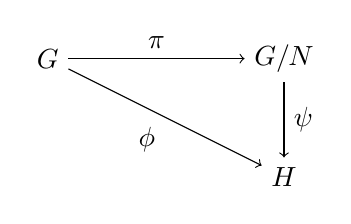
\begin{tikzpicture}
        \node (G) at (0, 0) {$G$};
        \node (GN) at (3, 0) {$G/N$};
        \node (H) at (3, -1.5) {$H$};
        \draw[->] (G) to node[above] {$\pi$} (GN);
        \draw[->] (G) to node[below left] {$\phi$} (H);
        \draw[->] (GN) to node[right] {$\psi$} (H);
    \end{tikzpicture}
\end{center}

\newpage

\subsection{Composition Series and the H\"older Program} \label{sec3.4}

\prop[Cauchy's Theorem for Abelian Groups] \label{prop3.21}
Let $G$ be finite abelian with prime $p$ dividing $|G|$. Then there exists $g \in G$ where $|g| = p$.

\begin{proof}
    Induct on $|G|$. Suppose $|G| > 1$ and $g \in G$ with $g \neq 1$. If $|G| = p$, then $|g| = p$ by Lagrange's. If $|G| > p$ and $p$ divides $|g|$, then $|g| = kp$ for $k \in \zp$, hence $|g^k| = p$ by \autoref{prop2.5}.

    Suppose $p$ does not divide $|g|$, and put $N = \gen g$. Since $G$ is abelian, $N \nsub G$, and Lagrange's shows that $|G/N| = |G|/|N|$ with $|G/N| < |G|$. Since $p$ does not divide $|N|$, then $p$ divides $|G/N|$. By the inductive hypothesis, there exists $\bar h \in G/N$ with $|\bar h| = p$. Note that $h \not\in N$ while $h^p \in N$ since $|\bar h| = p$, $\gen{h^p} \neq \gen h$, or $|h^p| < |h|$. By \autoref{prop2.5}, we have $p$ divides $|h|$. The proof is finished by the first case.
\end{proof}

\defi A (finite/infinite) group $G$ is \textbf{simple} if $G \neq 1$ and the only normal subgroups of $G$ are $1$ and $G$.

\defi Let $G$ be a group with a sequence of subgroups
\[1 = N_0 \leq N_1 \leq \cdots \leq N_{s - 1} \leq N_s = G\]
such that $N_i \nsub N_{i + 1}$ and $N_{i + 1}/N_i$ is simple for every $0 \leq i < s$. Then the sequence is a \textbf{composition series} of $G$. Moreover, the quotient groups $N_{i + 1}/N_i$ are called the \textbf{composition factors} of $G$.

\theo[Jordan--H\"older] \label{theo3.22}
Let $G$ be nontrivial and finite. Then
\begin{enumerate}
    \item $G$ has a composition series, and
    \item the composition factors in a composition series are unique in that if
    \[1 = N_0 \leq N_1 \leq \cdots \leq N_{s - 1} \leq N_s = G, \quad 1 = M_0 \leq M_1 \leq \cdots \leq M_{t - 1} \leq M_t = G\]
    are two composition series of $G$, then $s = t$ and there exists a permutation $\pi$ of $\set{1, 2, \ldots, s}$ such that $N_{i + 1}/N_i \cong M_{\pi(i) + 1}/M_{\pi(i)}$ for all $i$.
\end{enumerate}

\begin{proof}
    See Exercises 3.4.6, 3.4.9, and 3.4.10.
\end{proof}

\defi The \textbf{H\"older Program} is the program:
\begin{enumerate}
    \item Classify all simple groups, and
    \item Use the classification of simple groups to classify all finite groups by the Jordan--H\"older Theorem.
\end{enumerate}

\noindent \textcolor{Plum}{{\large$\heartsuit$} \squad \textsc{Theorem: The Classification of Finite Simple Groups}}

There are 18 infinite families of finite simple groups, and 26 sporadic finite simple groups such that every finite simple group is isomorphic to exactly one of these groups.

\noindent \textcolor{Plum}{{\large$\heartsuit$} \squad \textsc{Theorem: Feit--Thompson}}

Every finite simple group of odd order is isomorphic to $Z_p$ for some prime $p$.

\defi A group $G$ is \textbf{solvable} if there is a chain of subgroups
\[1 = H_0 \nsub H_1 \nsub \cdots \nsub H_{n - 1} \nsub H_n = G\]
such that $H_{i + 1}/H_i$ is abelian for every $0 \leq i < n$.

\noindent \textcolor{Plum}{{\large$\heartsuit$} \squad \textsc{Theorem: Hall's Theorem and its Converse}}

A finite group $G$ is solvable if and only if for every divisor $n$ of $|G|$ such that $\gcd(n, |G|/n) = 1$, there exists a subgroup $H \leq G$ such that $|H| = n$.

\ex We claim for any group $G$ with $N \nsub G$ solvable and $G/N$ solvable, then $G$ is solvable. Let $1 = N_0 \nsub N_1 \nsub \cdots N_n = N$ be a chain of subgroups such that $N_{i + 1}/N_i$ is abelian for every $0 \leq i < n$. Let $\bar 1 = \bar{H_0} \nsub \bar{H_1} \nsub \cdots \nsub \bar{H_m} = G/N$ be a chain of subgroups such that $\bar{H_{i + 1}}/\bar{H_i}$ is abelian for every $0 \leq i < m$. By the Fourth Isomorphism Theorem, there are subgroups $H_i$ with $N \leq H_i$ such that $\bar{H_i} = H_i/N$. The Third Isomorphism Theorem shows that
\[\bar{H_{i + 1}}/\bar{H_i} \cong H_{i + 1}/H_i\]
Then
\[1 = N_0 \nsub N_1 \nsub \cdots N_n = N = H_0 \nsub H_1 \nsub \cdots \nsub H_m = G\]
is a chain of subgroups with abelian successive quotients, hence $G$ is solvable.

\newpage

\subsection{Transpositions and the Alternating Group} \label{sec3.5}

\defi A \textbf{transposition} is a 2-cycle. In particular, any $(a_1\ a_2 \cdots a_k)$ with $k \geq 2$ can be written as a product of $k - 1$ transpositions:
\[(a_1\ a_2 \cdots a_k) = (a_1\ a_k)(a_1\ a_{k - 1}) \cdots (a_1\ a_2)\]

\defi Let $a_1, a_2, \ldots, a_n$ be independent symbols, and consider the \textbf{Vandermonde Polynomial} in $a_1, a_2, \ldots, a_n$ defined by
\[\Delta = \prod_{1 \leq i < j \leq n} (a_i - a_j)\]
Let $\sigma \in S_n$ act on $\Delta$ by permuting the subscripts of $a_i$. Then $\sigma(\Delta) = \pm 1 \Delta$. Define the \textbf{sign} of $\sigma$ to be
\[\ep(\sigma) =
\begin{cases}
    1 & \text{if $\sigma(\Delta) = +1 \Delta$} \\
    -1 & \text{if $\sigma(\Delta) = -1 \Delta$}
\end{cases}\]
An \textbf{even} permutation is when $\ep(\sigma) = 1$, and an \textbf{odd} permutation is when $\ep(\sigma) = -1$.

\prop[Sign is Homomorphism] \label{prop3.23}
The map $\ep : S_n \to \set{\pm 1}$ is a homomorphism, where $\set{\pm 1} \cong Z_2$.
\begin{proof}
    For $\tau, \sigma \in S_n$, we have
    \[(\tau\sigma)(\Delta) = \prod_{1 \leq i < j \leq n}(a_{\tau\sigma(i)} - a_{\tau\sigma(j)})\]
    If $\sigma(\Delta)$ has $k$ factors switched, then $\ep(\sigma) = (-1)^k$. There are $k$ factors of the form $a_{\tau\sigma(i)} - a_{\tau\sigma(j)}$ with $\tau\sigma(i) > \tau\sigma(j)$, and $\tau$ switches these factors if and only if $\tau(i) > \tau(j)$, so that $\ep(\tau\sigma) = (-1)^k\ep(\tau) = \ep(\sigma)\ep(\tau)$.
\end{proof}

\prop[Transpositions are Odd, $\ep$ is Surjective] \label{prop3.24}
\begin{proof}
    Note that $\ep((1\ 2)) = -1$. For any $(i\ j)$ with $1 \leq i < j \leq n$, let $\sigma \in S_n$ such that $\sigma(1) = i$ and $\sigma(2) = j$. Then $\ep((i\ j)) = \ep(\sigma(1\ 2)\sigma\inv) = \ep(\sigma)\ep((1\ 2))\ep(\sigma\inv) = -1$. Moreover, $\ep$ is surjective since $\ep((1\ 2)) = -1$ and $\ep(\id) = 1$.
\end{proof}

\note A useful conjugation formula is $\sigma(i\ j)\sigma\inv = (\sigma(i)\ \sigma(j))$ for $\sigma \in S_n$ and $1 \leq i < j \leq n$.

\defi The \textbf{alternating group} $A_n$ is the set of even permutations in $S_n$, or $\ker\ep$. By the First Isomorphism Theorem, then $A_n \nsub S_n$ and $S_n/A_n \cong Z_2$, hence $|A_n| = n!/2$.

\prop[Odd Permutation If and Only If Odd Number of Even Length Cycles] \label{prop3.25}
A permutation $\sigma$ is odd if and only if the number of cycles of even length in its disjoint cycle decomposition is odd.
\begin{proof}
    For $\sigma \in S_n$ with cycle decomposition $\sigma_1\sigma_2 \cdots \sigma_k$, then $\ep(\sigma) = \ep(\sigma_1)\ep(\sigma_2) \cdots \ep(\sigma_k)$. For $\ep(\sigma) = -1$, there must be an odd number of $\sigma_i$ with $\ep(\sigma_i) = -1$, or an odd number of cycles of even length in the cycle decomposition. Conversely, an odd number of cycles of even length in the cycle decomposition implies $\ep(\sigma) = -1$.
\end{proof}

\ex We claim the subgroup lattice of $A_4$ is as follows:
\begin{center}
    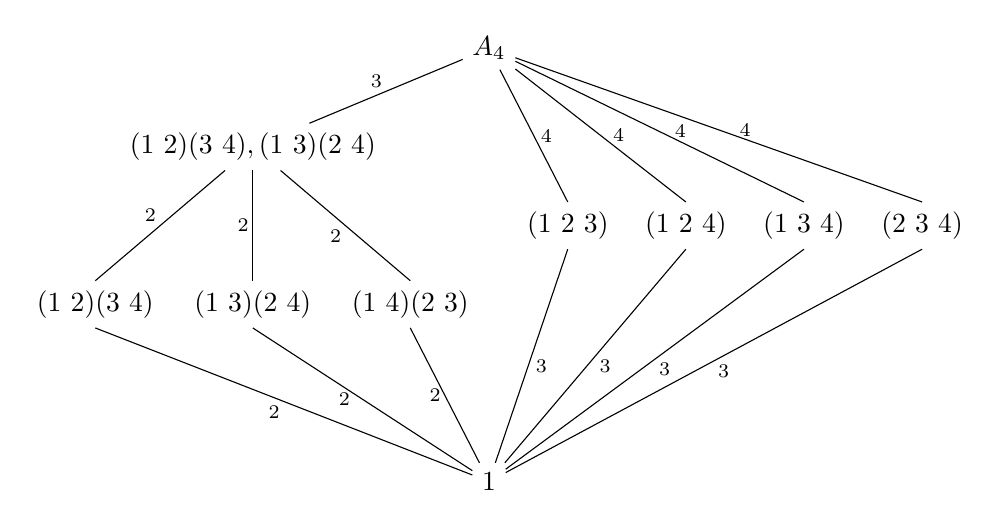
\begin{tikzpicture}
        \node (a4) at (0, 0.25) {$A_4$};

        \node (v4) at (-3, -1) {$\gen{(1\ 2)(3\ 4), (1\ 3)(2\ 4)}$};

        \node (123) at (1, -2) {$\gen{(1\ 2\ 3)}$};
        \node (124) at (2.5, -2) {$\gen{(1\ 2\ 4)}$};
        \node (134) at (4, -2) {$\gen{(1\ 3\ 4)}$};
        \node (234) at (5.5, -2) {$\gen{(2\ 3\ 4)}$};

        \node (1234) at (-5, -3) {$\gen{(1\ 2)(3\ 4)}$};
        \node (1324) at (-3, -3) {$\gen{(1\ 3)(2\ 4)}$};
        \node (1423) at (-1, -3) {$\gen{(1\ 4)(2\ 3)}$};

        \node (1) at (0, -5.25) {1};

        \draw (1) -- (1234.south) node [midway, below left=-2pt] {\scriptsize 2};
        \draw (1234.north) -- (v4) node [midway, above left=-2pt] {\scriptsize 2} -- (a4) node [midway, above left=-2pt] {\scriptsize 3};
        \draw (1) -- (1324.south) node [midway=, left=1pt] {\scriptsize 2};
        \draw (1324.north) -- (v4) node [midway, left=-2pt] {\scriptsize 2};
        \draw (1) -- (1423.south) node [midway, left=-2pt] {\scriptsize 2};
        \draw (1423.north) -- (v4) node [midway, below left=-2pt] {\scriptsize 2};
        \draw (1) -- (123.south) node [midway, below right=-2pt] {\scriptsize 3};
        \draw (123.north) -- (a4) node [midway, right=-1pt] {\scriptsize 4};
        \draw (1) -- (124.south) node [midway, below right=-2pt] {\scriptsize 3};
        \draw (124.north) -- (a4) node [midway, right=1pt] {\scriptsize 4};
        \draw (1) -- (134.south) node [midway, below right=-2pt] {\scriptsize 3};
        \draw (134.north) -- (a4) node [midway, right=2pt] {\scriptsize 4};
        \draw (1) -- (234.south) node [midway, below right=-2pt] {\scriptsize 3};
        \draw (234.north) -- (a4) node [midway, right=4pt] {\scriptsize 4};
    \end{tikzpicture}
\end{center}